%% Continuation of Task 1.5 for the main notes document.
%% Drop-in replacement starting at "\paragraph{Pairing Price and Demand data}".
%% Assumes the preamble of the main notes (\bp, \bd, \bx, \bs, \bxi, lstlisting, ...).

\paragraph{Pairing price and demand data}
\mbox{}\\

The price data is from 2026 while the demand data is from 2018, so the two series
cannot be matched on the full calendar date. We instead match on the (month, day)
pair only: each of the nine price days is paired with the demand profile recorded
on the same month and day of 2018. This gives
\begin{equation}
    \xi_i = (\bp^i, \bd^i), \qquad i=1,\dots,N, \qquad N = 9,
\end{equation}
covering 8--16 September. The remaining $365-9=356$ demand profiles are not used.
Table~\ref{tab:profiles} summarises the nine paired profiles.

\begin{table}[h]
  \centering
  \caption{Summary of the $N=9$ daily profiles (bus \texttt{ADK\_V\_C}).}
  \label{tab:profiles}
  \begin{tabular}{l|rrr|rr}
    \hline
    Date & Mean price & Peak price & Min price & Total demand & Peak demand \\
         & (\$/MWh)   & (\$/MWh)   & (\$/MWh)  & (MWh)        & (MW)        \\
    \hline
    08 Sep & 42.50 &  84.59 & 23.58 & 10.80 & 0.539 \\
    09 Sep & 46.55 & 103.14 & 24.44 &  8.39 & 0.417 \\
    10 Sep & 46.14 &  96.01 & 23.01 & 14.32 & 0.801 \\
    11 Sep & 34.04 &  53.47 & 23.79 & 14.51 & 0.801 \\
    12 Sep & 31.14 &  54.03 & 17.30 & 14.52 & 0.801 \\
    13 Sep & 32.00 &  56.52 & 18.06 & 14.35 & 0.801 \\
    14 Sep & 31.97 &  49.54 & 20.84 & 13.68 & 0.776 \\
    15 Sep & 33.84 &  60.09 & 18.99 & 10.60 & 0.529 \\
    16 Sep & 42.72 &  72.64 & 25.45 &  8.24 & 0.408 \\
    \hline
  \end{tabular}
\end{table}

Two features of the data matter for what follows. First, prices vary by a factor
of three or more within a single day (for example \$23.01 to \$96.01/MWh on
10 September), which is exactly the spread a battery can exploit. Second, the
demand of an inference data center is comparatively flat: the facility never
switches off, so $\bd^i$ stays within a narrow band and the total daily energy is
only 8--15~MWh. The savings therefore come almost entirely from the price signal
rather than from the shape of the demand.

\subsection{Evaluating the cost for a given capacity}

For a profile $\xi = (\bp, \bd)$ and a battery capacity $B \ge 0$ (in MWh), the
optimal daily cost is the optimal value of~\eqref{p:battery-control},
\begin{subequations}
\label{p:Q}
\begin{align}
    Q(B,\xi) \;=\; \min_{x_t \ge 0,\, s_t \ge 0} \quad & \sum_{t\in[T]} p_t x_t\\
    \text{s.t.}\quad & s_t = s_{t-1} + x_t - d_t, && \forall t\in[T],\\
                     & x_t \ge d_t - s_{t-1},     && \forall t\in[T],\\
                     & s_t \le B,                 && \forall t\in [T],
\end{align}
\end{subequations}
with $T=24$ and $s_0 = 0$, i.e.\ the battery starts each day empty and no energy
is carried over between days.

A few properties are worth noting before looking at the numbers.
\begin{itemize}
  \item The problem is a linear program in $48$ variables, and it is feasible for
        every $B\ge 0$ (take $x_t = d_t$, $s_t = 0$) and bounded below by $0$.
  \item When $B=0$ the storage constraint forces $s_t = 0$, so the only feasible
        choice is $x_t = d_t$ and $Q(0,\xi) = \bp^\top \bd$. This is the
        \emph{no-battery} benchmark: buy exactly what is needed, when it is needed.
  \item Increasing $B$ only relaxes the constraint $s_t \le B$, so the feasible set
        grows and $Q(B,\xi)$ is non-increasing in $B$. Moreover $Q(\cdot,\xi)$ is
        the optimal value of an LP in which $B$ appears on the right-hand side, so
        it is convex in $B$; the same then holds for the average $C_N(\cdot)$.
\end{itemize}

The model ignores charging and discharging losses, charge/discharge power limits,
degradation, the capital cost of the battery, and the possibility of selling energy
back to the grid. It therefore gives an upper bound on the savings a real battery
of the same capacity would deliver.

\begin{lstlisting}
def solve_battery_lp(p: np.ndarray, d: np.ndarray, B: float) -> float:
    """Q(B, xi): optimal cost of meeting demand d at prices p with capacity B."""
    x = cp.Variable(T, nonneg=True)  # energy bought from the grid each hour
    s = cp.Variable(T, nonneg=True)  # battery state of charge each hour

    constraints = []
    for t in range(T):
        s_prev = 0 if t == 0 else s[t-1]
        constraints.append(s[t] == s_prev + x[t] - d[t])
        constraints.append(x[t] >= d[t] - s_prev)
        constraints.append(s[t] <= B)

    problem = cp.Problem(cp.Minimize(p @ x), constraints)
    problem.solve()
    return problem.value
\end{lstlisting}

\subsection{Sample average cost and the capacity sweep}

Fixing $B$ and solving~\eqref{p:Q} once for each of the $N$ profiles gives the
sample average daily cost
\begin{equation}
    C_N(B) = \frac{1}{N}\sum_{i\in[N]} Q(B,\xi_i).
\end{equation}
We repeat this over the capacity grid $B \in \{0, 0.5, 1.0, \dots, 15\}$~MWh
($31$ values), always using the same nine profiles, which amounts to
$31\times 9 = 279$ linear programs.

\begin{lstlisting}
def sample_average_cost(xis: list[dict], B: float) -> float:
    """C_N(B): mean of Q(B, xi_i) over the N days in xis."""
    return float(np.mean([solve_battery_lp(xi["p"], xi["d"], B) for xi in xis]))


B_VALUES = np.linspace(0, 15, 31)
C_N = np.array([sample_average_cost(xis, B) for B in B_VALUES])
\end{lstlisting}

\subsection{Results}

Figure~\ref{fig:cost} plots $C_N(B)$ against $B$, and Table~\ref{tab:results}
lists the values at selected capacities.

\begin{figure}[h]
  \centering
  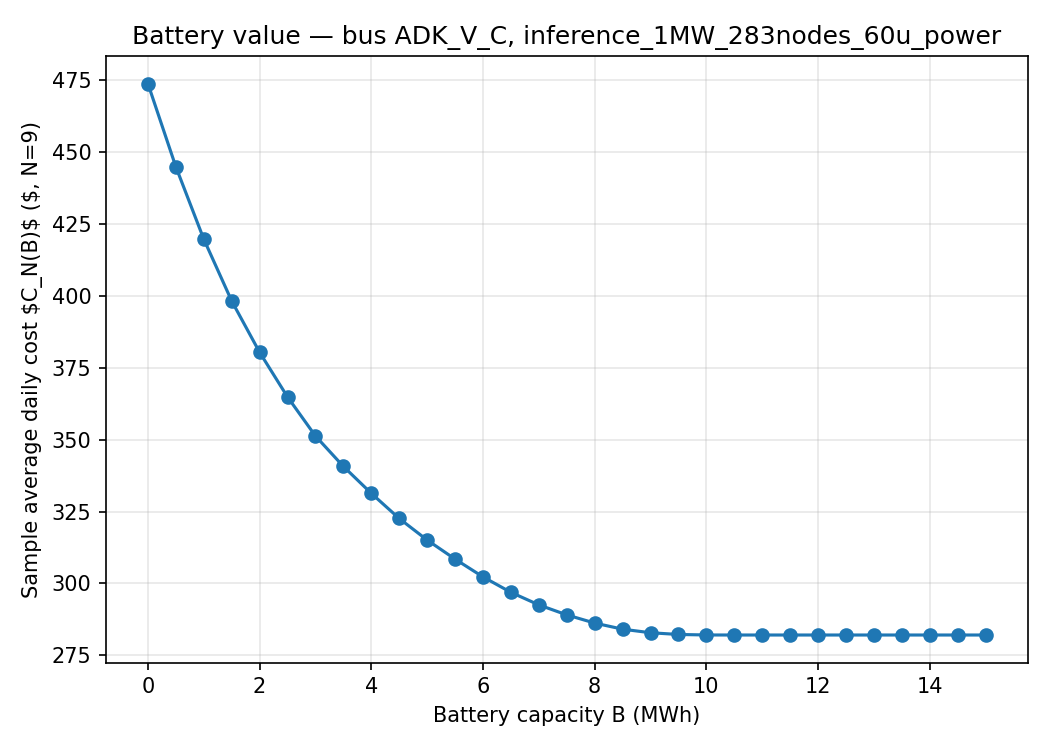
\includegraphics[width=0.7\textwidth]{task_1.5/visualizations/cost_vs_battery_capacity.png}
  \caption{Sample average daily cost $C_N(B)$ against battery capacity $B$, over
    $N=9$ days (8--16 September) at bus \texttt{ADK\_V\_C}.}
  \label{fig:cost}
\end{figure}

\begin{table}[h]
  \centering
  \caption{Sample average daily cost $C_N(B)$ for selected capacities.}
  \label{tab:results}
  \begin{tabular}{r|rr}
    \hline
    $B$ (MWh) & $C_N(B)$ (\$) & Reduction vs.\ $B=0$ \\
    \hline
     0.0 & 473.76 &  0.0\% \\
     1.0 & 419.72 & 11.4\% \\
     2.0 & 380.37 & 19.7\% \\
     3.0 & 351.26 & 25.9\% \\
     4.0 & 331.33 & 30.1\% \\
     5.0 & 315.09 & 33.5\% \\
     6.0 & 302.28 & 36.2\% \\
     7.0 & 292.54 & 38.3\% \\
     8.0 & 286.22 & 39.6\% \\
     9.0 & 282.86 & 40.3\% \\
    10.0 & 282.09 & 40.5\% \\
    $\ge 10.15$ & 282.07 & 40.5\% \\
    \hline
  \end{tabular}
\end{table}

Without storage the average daily cost is
\begin{equation}
    C_N(0) = \frac{1}{N}\sum_{i\in[N]} (\bp^i)^\top \bd^i = \boxed{\$473.76},
\end{equation}
and with enough storage it falls to
\begin{equation}
    \lim_{B\to\infty} C_N(B) = \boxed{\$282.07},
\end{equation}
a reduction of $40.5\%$.

The curve is decreasing and convex, as predicted above. The first megawatt-hour of
capacity is worth about \$54 per day, the second about \$39, the fifth about \$16,
and the tenth less than \$1. The reason is that each additional unit of capacity is
used to shift a progressively less profitable megawatt-hour: the optimizer first
moves energy out of the most expensive hour into the cheapest one that precedes it,
and once that arbitrage is exhausted it must settle for pairs of hours with a
smaller price gap.

Beyond $B \approx 10.15$~MWh the cost is flat at \$282.07. At that point the
constraint $s_t \le B$ is slack on all nine days, so every unit of demand is
already being met at the cheapest price available at or before the hour it is
needed, and extra capacity buys nothing. The saturating capacity is on the order of
one day of total demand (8--15~MWh in Table~\ref{tab:profiles}), which is what one
would expect: since the battery cannot carry energy across days, it can never need
to hold more than a single day's consumption. This flat region is an artefact of
the cost-free battery assumption --- once the capital cost of storage is included,
the optimal capacity sits where the marginal saving per MWh equals the amortised
marginal cost, well to the left of the saturation point.

Table~\ref{tab:days} breaks the result down by day, comparing the no-battery cost
with the cost at $B=15$~MWh (i.e.\ in the saturated regime).

\begin{table}[h]
  \centering
  \caption{Daily optimal cost $Q(B,\xi_i)$ with no battery and with $B=15$~MWh.}
  \label{tab:days}
  \begin{tabular}{l|rrr}
    \hline
    Date & $Q(0,\xi_i)$ (\$) & $Q(15,\xi_i)$ (\$) & Saving \\
    \hline
    08 Sep & 472.70 & 276.69 & 41.5\% \\
    09 Sep & 408.76 & 219.04 & 46.4\% \\
    10 Sep & 719.32 & 355.27 & 50.6\% \\
    11 Sep & 513.21 & 376.02 & 26.7\% \\
    12 Sep & 481.11 & 276.22 & 42.6\% \\
    13 Sep & 481.97 & 291.43 & 39.5\% \\
    14 Sep & 456.58 & 301.24 & 34.0\% \\
    15 Sep & 366.69 & 217.66 & 40.6\% \\
    16 Sep & 363.51 & 225.10 & 38.1\% \\
    \hline
    Mean   & 473.76 & 282.07 & 40.5\% \\
    \hline
  \end{tabular}
\end{table}

The value of the battery varies substantially across days, and it tracks the
intraday price spread rather than the price level. The best day is 10 September
(\$364 saved, $50.6\%$), which has both high demand and the widest spread
(\$23.01--\$96.01/MWh). The worst is 11 September ($26.7\%$), where demand is
essentially the same but prices stay in the narrow band \$23.79--\$53.47/MWh, so
there is much less to arbitrage. This is the practical point of the exercise: the
battery is paid for by price volatility, not by the average price level.

\subsection{Limitations}

The sample is small ($N=9$) and covers one week in September, so $C_N(B)$ is a
noisy estimate of the true expected cost and says nothing about seasonal effects.
The demand is simulated 2018 data paired with real 2026 prices on (month, day)
alone, so any genuine correlation between load and price --- which is precisely
what makes storage valuable on hot days in ERCOT --- is absent by construction.
The results are also specific to one bus and one utilization profile. Finally, as
noted above, the model omits losses, power limits and capital cost, so the reported
savings should be read as an upper bound.
